\chapter{Datasets\label{sec:datasets}}

This thesis is based on five different already existing datasets.
This chapter discusses these datasets based on different criteria:

\begin{description}
    \item[source:] reference of the owner of the dataset and brief description of the original purpose of the dataset. Importantly, this part also discusses the source of the annotation.
    \item[Patient sample:] statistics of the patients whose medical images were collected such as age, gender and possible spine pathologies.
    \item[Technical information:] discusses the imaging technology, the image resolution and the spatial dimensions of the image. 
\end{description}

\section{Global dataset overview}

\todo[inline]{Overview of the datasets gathered. MRI / CT, number of images, type of annotation + WHO performed the annotation? Was it a medical doctor or one of the researchers?}

\begin{SCtable}[\sidecaptionrelwidth][h]
 
    \begin{tabular}{ l l l l l} 
     \hline
     \hline
     Name & reference & imaging & Quantity & Annotation \\
          &           & technology & [images] & \\
     \hline 
    UWSpine & \cite{Glocker}  & \acrshort{ct} & 125 & point  \\ 
    xVertSeg & \cite{Ibragimov2014, Korez2015} & \acrshort{ct} & 15 & full \\
    UniSiegen  & \cite{Zukic2014} & \acrshort{mri} & 17 & full \\
    PLoS & \cite{Chu2015} & \acrshort{mri} & 23 & semantic \\
    MyoSegmenTUM & \cite{Burian2019} & \acrshort{mri} &  54 & full \\
     \hline
     \hline
    \end{tabular}
    \caption{List of dataset references. For more details on the data quantity, please consult chapter \ref{seg:datasetcomparison}. 
    Notably, the fact that some images were taken from the same patient is important to recognize. It means the dataset is grouped. 
    The agreement with prof. T. Vrtovec regarding the xVertSeg dataset can be found in appendix \ref{seg:datasetagreement}.}

\end{SCtable}

\begin{SCtable}[\sidecaptionrelwidth][h]
 
    \begin{tabular}{ l l l l} 
     \hline
     \hline
     Name & X & Y & Z \\
     \hline 
    UWSpine & Left-right & Anteroposterior & Craniocaudal \\
    xVertSeg & Left-right & Anteroposterior & Craniocaudal \\
    UniSiegen  &  Anteroposterior & Craniocaudal & Left-right \\
    PLoS & Left-right & Anteroposterior & Craniocaudal$^\dagger$ \\
    MyoSegmenTUM &  Anteroposterior & Craniocaudal & Left-right \\
     \hline
     \hline
    \end{tabular}
    \caption{List of dataset references. For more details on the data quantity, please consult chapter \ref{seg:datasetcomparison}. 
    $^\dagger$ The Craniocaudal axis in the PLoS dataset is inverted.}

\end{SCtable}

\begin{SCfigure}[][htb]
    \centering
    \begin{minipage}{.45\textwidth}
        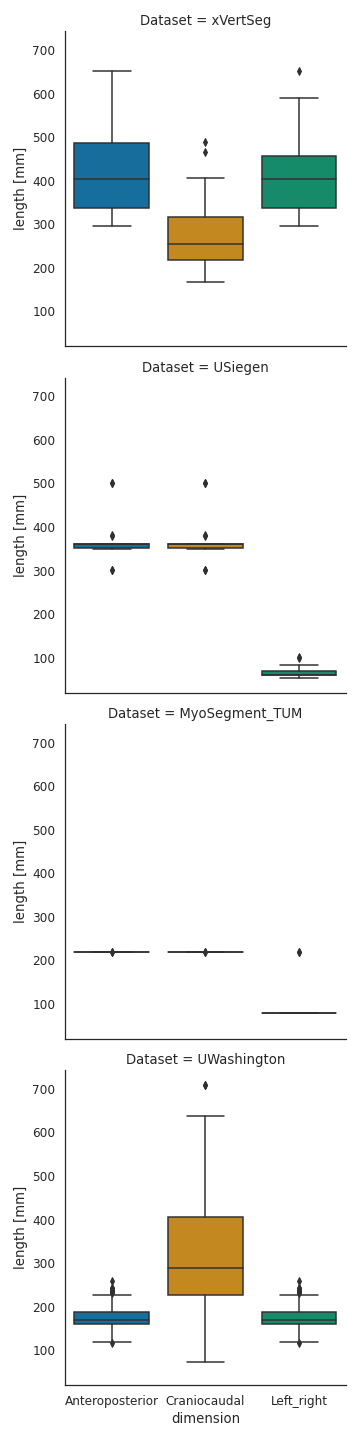
\includegraphics[width=.98\textwidth]{automated_graphs/AllDataset_DimensionsBoxplot.png}
    \end{minipage}%
    \begin{minipage}{0.45\textwidth}
        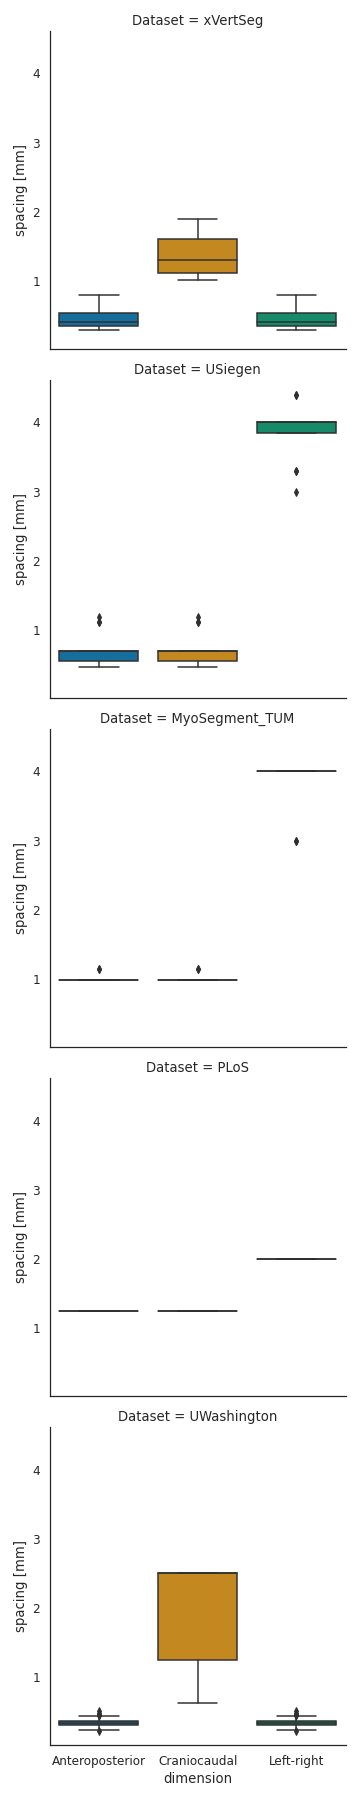
\includegraphics[width=.98\textwidth]{automated_graphs/AllDataset_SpacingBoxplot.png}
    \end{minipage}
    \caption{Boxplots comparing the scan dimensions and initial resolution of the different datasets.}
    \label{fig:AllDataset_dims}
\end{SCfigure}

\section{Comparison of the different datasets\label{seg:datasetcomparison}}


\subsection{xVertSeg\label{sec:xVertSeg}}



The xVertSeg \cite{Ibragimov2012, xxx} was kindly made available by prof. T. Vrtovec (University of Ljubljana, Faculty of Electrical Engineering, Slovenia), see appendix \ref{seg:datasetagreement} for the agreement.
This dataset contains 25 \acrfull{ct} scans of the lumbar spine, of which 15 \acrshort{ct} scans are fully labeled.
Given the provided data, I can assume these 15 scans were collected from 15 different patients.

For each of these 15 scans, full instance segmenation masks for all 5 lumbar vertebrae are provided. The delineation was performed by a skilled professional.

Additionally, for each vertebra a fracture class and fracture grade is provided. 
Apart from vertebrae classified as \textit{normal}, the dataset contains \textit{mild}, \textit{moderate} and \textit{severe} cases of vertebrae fracture types \textit{wedge}, \textit{crush} and \textit{biconcavity}.
\marginpar{
        % This file was created by tikzplotlib v0.9.8.
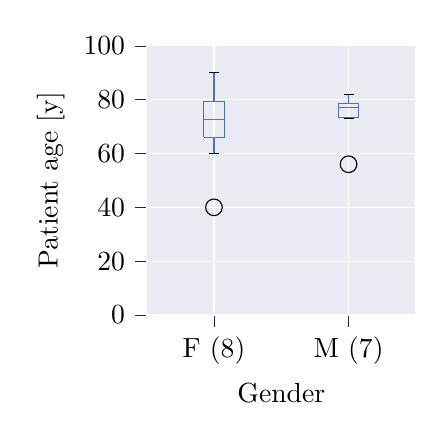
\begin{tikzpicture}

\definecolor{color0}{rgb}{0.917647058823529,0.917647058823529,0.949019607843137}
\definecolor{color1}{rgb}{0.298039215686275,0.447058823529412,0.690196078431373}
\definecolor{color2}{rgb}{0.768627450980392,0.305882352941176,0.32156862745098}

\begin{axis}[
axis background/.style={fill=color0},
axis line style={white},
height=5cm,
tick align=outside,
tick pos=left,
width=5cm,
x grid style={white},
xlabel={Gender},
xmajorgrids,
xmin=0.5, xmax=2.5,
xtick style={color=white!15!black},
xtick={1,2},
xticklabels={F (8),M (7)},
y grid style={white},
ylabel={Patient age [y]},
ymajorgrids,
ymin=0, ymax=100,
ytick style={color=white!15!black}
]
\addplot [color1, opacity=1]
table {%
0.925 66
1.075 66
1.075 79.25
0.925 79.25
0.925 66
};
\addplot [color1, opacity=1]
table {%
1 66
1 60
};
\addplot [color1, opacity=1]
table {%
1 79.25
1 90
};
\addplot [black, opacity=1]
table {%
0.9625 60
1.0375 60
};
\addplot [black, opacity=1]
table {%
0.9625 90
1.0375 90
};
\addplot [black, mark=o, mark size=3, mark options={solid,fill opacity=0}, only marks]
table {%
1 40
};
\addplot [color1, opacity=1]
table {%
1.925 73.5
2.075 73.5
2.075 78.5
1.925 78.5
1.925 73.5
};
\addplot [color1, opacity=1]
table {%
2 73.5
2 73
};
\addplot [color1, opacity=1]
table {%
2 78.5
2 82
};
\addplot [black, opacity=1]
table {%
1.9625 73
2.0375 73
};
\addplot [black, opacity=1]
table {%
1.9625 82
2.0375 82
};
\addplot [black, mark=o, mark size=3, mark options={solid,fill opacity=0}, only marks]
table {%
2 56
};
\addplot [color2, opacity=1]
table {%
0.925 72.5
1.075 72.5
};
\addplot [color2, opacity=1]
table {%
1.925 77
2.075 77
};
\end{axis}

\end{tikzpicture}

        \captionof{figure}{xVertSeg patients age distribution}
        \label{fig:xVertSeg_Age}
    }

\subsubsection{Original Objective of the Dataset}

The objective of the \textit{xVertSeg challenge}\footnote{see \url{http://lit.fe.uni-lj.si/xVertSeg/database.php}} (2015) was organized by the University of Ljubljana.
Based on the 15 provided scans with corresponding masks, the participans were required to construct a model to make predictions on the test set of 10 unlabelled scans.

The challenge consisted of two tasks:
\begin{enumerate}
    \item Segmentation of the lumbar vertebrae. For each scan in the test set, the segmentation masks of the lumbar vertebrae were requested.
    \item Fracture classification on the segmented vertebrae, consisting of morphological grade and fracture classification.
\end{enumerate}

\subsubsection{Patient statistics}

The patients in the xVertSeg dataset train set consist of 8 females and 7 males.
The age of these patients is slightly higher than for the other datasets.
The average patient in this dataset is 71 years old.
A box plot of the age distribution between genders is shown in figure \ref{fig:xVertSeg_Age}. 

\begin{SCtable}[\sidecaptionrelwidth][h]
    \centering
        \begin{tabular}{lrrrrrr}
\toprule
{} &  L1 &  L2 &  L3 &  L4 &  L5 &  Total \\
\midrule
biconcave &   6 &   7 &   8 &   4 &   2 &     27 \\
normal    &   5 &   6 &   4 &   4 &   7 &     26 \\
wedge     &   3 &   2 &   2 &   3 &   2 &     12 \\
crush     &   1 &   0 &   1 &   4 &   4 &     10 \\
\bottomrule
\end{tabular}

        \caption{Every patient in the xVertSeg dataset suffers from at least one spine pathology.
        Most of these pathologies are identified as \textit{mild}.
        This table counts the spine pathologies and normal vertebrae observed over all 15 patients in the xVertSeg dataset.}   
\end{SCtable}

\subsubsection{Technical information}

The xVertSeg dataset contains 15 \acrshort{ct} annotated scans. 
This dataset is very interesting due to the high quality and high resolution of the images.
On figure \ref{fig:xVertSeg_image002}, two slices of the same patient (002) are represented.
The slices show the complete, uncropped sections of the torso and abdominal region of the patient. 
There is no \acrshort{roi} cropping.

\begin{SCfigure}[][htb]
    \centering
    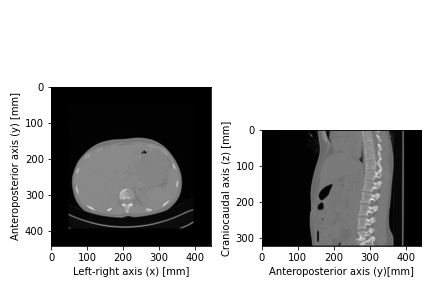
\includegraphics[width=.95\textwidth]{automated_graphs/xVertSeg_image002.png}
    \caption{xVertSeg scan \textit{image002}. \label{fig:xVertSeg_image002}}
\end{SCfigure}

The distribution of the scan dimensions is shown in figure \ref{fig:AllDataset_dims}. This also illustrates the \textit{xVertSeg} dataset consists of large, high resolution images.
Mind that during pre-processing the scans are resampled on a $1mm \times 1mm \times 1mm$ grid.


\subsection{UniSiegen dataset\label{sec:DataUSiegen}}

This dataset is made available in 2014 by the University of Siegen, Germany.
Dr D. Zukic \cite{Zukic2014} constructed it as part of his PhD project.

\marginpar{
        % This file was created by tikzplotlib v0.9.8.
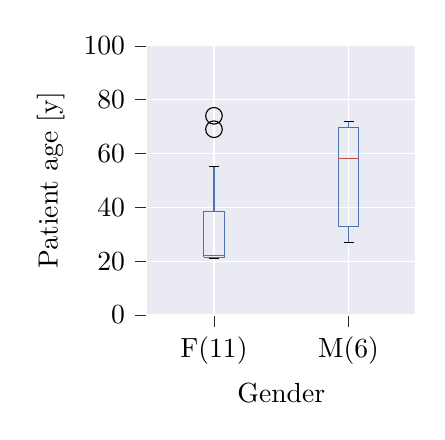
\begin{tikzpicture}

\definecolor{color0}{rgb}{0.917647058823529,0.917647058823529,0.949019607843137}
\definecolor{color1}{rgb}{0.298039215686275,0.447058823529412,0.690196078431373}
\definecolor{color2}{rgb}{0.768627450980392,0.305882352941176,0.32156862745098}

\begin{axis}[
axis background/.style={fill=color0},
axis line style={white},
height=5cm,
tick align=outside,
tick pos=left,
width=5cm,
x grid style={white},
xlabel={Gender},
xmajorgrids,
xmin=0.5, xmax=2.5,
xtick style={color=white!15!black},
xtick={1,2},
xticklabels={F(11),M(6)},
y grid style={white},
ylabel={Patient age [y]},
ymajorgrids,
ymin=0, ymax=100,
ytick style={color=white!15!black}
]
\addplot [color1, opacity=1]
table {%
0.925 21.5
1.075 21.5
1.075 38.5
0.925 38.5
0.925 21.5
};
\addplot [color1, opacity=1]
table {%
1 21.5
1 21
};
\addplot [color1, opacity=1]
table {%
1 38.5
1 55
};
\addplot [black, opacity=1]
table {%
0.9625 21
1.0375 21
};
\addplot [black, opacity=1]
table {%
0.9625 55
1.0375 55
};
\addplot [black, mark=o, mark size=3, mark options={solid,fill opacity=0}, only marks]
table {%
1 74
1 69
};
\addplot [color1, opacity=1]
table {%
1.925 33
2.075 33
2.075 69.5
1.925 69.5
1.925 33
};
\addplot [color1, opacity=1]
table {%
2 33
2 27
};
\addplot [color1, opacity=1]
table {%
2 69.5
2 72
};
\addplot [black, opacity=1]
table {%
1.9625 27
2.0375 27
};
\addplot [black, opacity=1]
table {%
1.9625 72
2.0375 72
};
\addplot [color2, opacity=1]
table {%
0.925 22
1.075 22
};
\addplot [color2, opacity=1]
table {%
1.925 58
2.075 58
};
\end{axis}

\end{tikzpicture}

        \captionof{figure}{USiegen patients age distribution}
        \label{fig:USiegen_Age}
    }

This dataset contains 26 \acrshort{mri} scans of 17 different patients\footnote{This is not clearly stated, but can be inferred from the metadata.}. 
The fact that scans of the same patient are correlated will be taken into account in the train, validation and test split.
For more details on this split, see section \ref{sec:trainValTestSplit} on page \pageref{sec:trainValTestSplit}.

\subsubsection{Original Objective of the Dataset}

This dataset was collected from several hospitals (Sarajevo, Marburg, Brisbane, Schwabach, Bad Wildungen \& Prague). The MRI scanner settings were varied between the scans (T1, T2, TIRM).
The PhD project objective was to build a segmentation model to automate the segmentation of the lumbar vertebrae in the \acrshort{mri} scans to facilitate the diagnosis of several spine pathologies 
such as scoliosis, spondylolisthesis \footnote{Spondylolisthesis is the displacement of one spinal vertebra compared to another.} and vertebral fractures.
The final model developed by dr. D. Zukic consisted of a Viola-Jones detector for detection and vertebral body size approximation.
The average Dice score compared to the manual reference was reported to be 79.3\%.

\subsubsection{Patient statistics}

In \cite{Zukic2014}, it is not entirely made clear which scans are taken from the same patient.
It is made clear, however that the 26 scans were not obtained from 26 patients.
The information was inferred from the naming of the scans and the provided gender en age information\footnote{
    Wrongfully assuming two scans come from the same patient does not cause data leakage.
}.

Figure \ref{fig:USiegen_Age} illustrates that the USiegen dataset contains almost double the number of female patients compared to male patients.
These patients are relatively young compared to the patients in the \textit{xVertSeg} dataset.

Only three of the patients in this dataset were categorized as having no spinal pathologies.

\subsubsection{Technical information}

Several \acrlong{mri} techniques were used to obtain the dataset: T1, T2 \& TIRM.
I do not take into account this factor in the model development or the dataset split.

The volumes in the USiegen dataset are strongly cropped. 
Both in the anteroposterior and the craniocaudal direction, the volumes are on average 370 mm.
In the left-right direction, however, the volumes have been cropped severely. The volumes are, on average, only 68 mm wide.
The images have been cropped to only include the \acrshort{roi}.
Along this left-right dimension, the voxel spacing is large. 

\begin{SCfigure}[][htb]
    \centering
    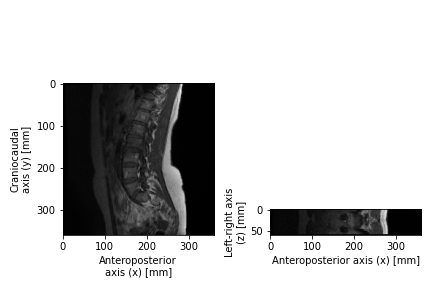
\includegraphics[width=.95\textwidth]{automated_graphs/USiegen_Aka3.png}
    \caption{USiegen dataset scan \textit{Aka3}. \label{fig:USiegen_Aka3}. It is immediately clear the USiegen volumes are cropped differently than the xVertSeg volumes.
    In the craniocaudal direction, both sacrum and coccyx are visible. Along the left-righ axis, the volumes have been cropped severely.}
\end{SCfigure}

The original scans in the \textit{USiegen} dataset were cropped in the \textit{left-right} direction. 
Although the scan resolution is relatively high in the Sagittal planes, the slice spacing along the left-right axis is coarser (see figure \ref{fig:AllDataset_dims}).  
\subsection{PLoS Dataset}

The \textit{PLoS} dataset was compiled for \cite{Chu2015} in 2015 by dr. C. Chu, University of Bern, Bern, Switzerland and made publically available \footnote{See : \url{ http://doi.org/10.5281/zenodo.22304 }} .
It consists of 23 T2-weighted spine \acrshort{mri} scans. 
Contrary to other datasets, the segmenation labels in this dataset do not provide information to destinguish the individual vertebrae from each other.

\subsubsection{Original Objective of the Dataset}

In \cite{Chu2015} the development of a random forest regression approach for spine vertebrae segmenation and classificiation is described.
The results of several random forest regressors and classifiers is unified with a voting mechanism.
This approach obtains a mean Dice metric score of 88.7\%.

\subsubsection{Patient statistics}

Due to the anomimization process, the \textit{PLoS} dataset does not contain patient information.
This means that it is not possible to produce any statistics regarding patient age or gender.

\subsubsection{Technical information}

As is indicated in figure \ref{fig:AllDataset_dims}, and in figure \ref{fig:PLoS_img02}, the PLoS image volumes are cropped in the left-right direction.
The volumes are consistently $381mm \times 381 mm \times 78 mm$, where the shortest dimension is in the left-right direction.

\begin{SCfigure}[][htb]
    \centering
    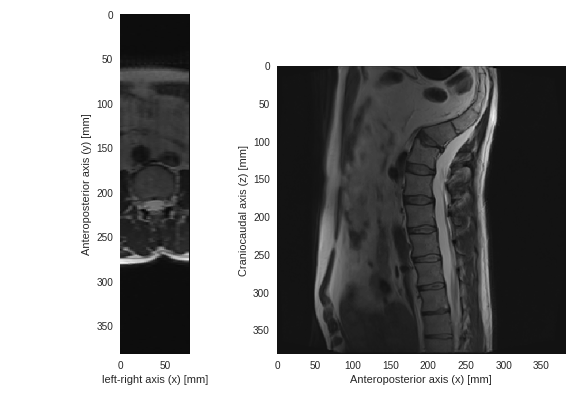
\includegraphics[width=.95\textwidth]{automated_graphs/PLoS_img02.png}
    \caption{
        PLoS dataset scan \textit{img02}. \label{fig:PLoS_img02}. The craniocaudal direction is cropped in a way comparable to the volumes in the USiegen dataset, but, the direction of this axis is inverted.
        The left-right axis is cropped similar to the USiegen data volumes.
    }
\end{SCfigure}
\subsection{MyoSegmenTUM datset}

This dataset is made available by S. Schläger from the Technische Universität München via the \acrfull{osf} \footnote{see \url{ https://osf.io/3j54b/?view_only=f5089274d4a449cda2fef1d2df0ecc56 }}.
It was constructed for the MyoSegmenTUM project \cite{Burian2019}.
It consists of 54 collections of \acrshort{mri} scans of the spine.
In this work, only the T2 weighted \acrlong{mri} scans are used.
The dataset also contains volumes with enhanced fat tissue response. Since the objective of this work is related to bone tissue rather than fat tissue, these volumes were not used.
Neither was the segmentation masks for the different dorsal muscles, which are also present in this dataset.

\subsubsection{Original Objective of the Dataset}

The MyoSegmenTUM Spine dataset is compiled as a reference dataset for developing segmentation algorithms of the lumbar spine vertebral bodies and muscle groups.
Information about this project can be found in \cite{Burian2019}.

\subsubsection{Patient statistics}

In figure \ref{fig:OSF_ageboxplot}, the age distribution of the patients in the MyoSegmenTUM dataset is shown.
There are more women (39) included in this dataset than men (15).
The male patients in this dataset are, on average, clearly younger than the female patients.

\marginpar{
        % This file was created by tikzplotlib v0.9.8.
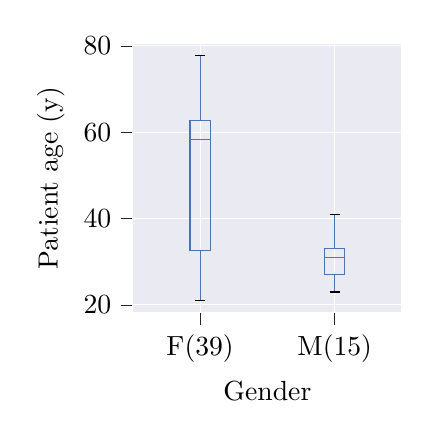
\begin{tikzpicture}

\definecolor{color0}{rgb}{0.917647058823529,0.917647058823529,0.949019607843137}
\definecolor{color1}{rgb}{0.298039215686275,0.447058823529412,0.690196078431373}
\definecolor{color2}{rgb}{0.768627450980392,0.305882352941176,0.32156862745098}

\begin{axis}[
axis background/.style={fill=color0},
axis line style={white},
height=5cm,
tick align=outside,
tick pos=left,
width=5cm,
x grid style={white},
xlabel={Gender},
xmajorgrids,
xmin=0.5, xmax=2.5,
xtick style={color=white!15!black},
xtick={1,2},
xticklabels={F(39),M(15)},
y grid style={white},
ylabel={Patient age (y)},
ymajorgrids,
ymin=18.1666324435318, ymax=80.5007186858316,
ytick style={color=white!15!black}
]
\addplot [color1, opacity=1]
table {%
0.925 32.5
1.075 32.5
1.075 62.7652292950034
0.925 62.7652292950034
0.925 32.5
};
\addplot [color1, opacity=1]
table {%
1 32.5
1 21
};
\addplot [color1, opacity=1]
table {%
1 62.7652292950034
1 77.6673511293635
};
\addplot [black, opacity=1]
table {%
0.9625 21
1.0375 21
};
\addplot [black, opacity=1]
table {%
0.9625 77.6673511293635
1.0375 77.6673511293635
};
\addplot [color1, opacity=1]
table {%
1.925 27
2.075 27
2.075 33
1.925 33
1.925 27
};
\addplot [color1, opacity=1]
table {%
2 27
2 23
};
\addplot [color1, opacity=1]
table {%
2 33
2 41
};
\addplot [black, opacity=1]
table {%
1.9625 23
2.0375 23
};
\addplot [black, opacity=1]
table {%
1.9625 41
2.0375 41
};
\addplot [color2, opacity=1]
table {%
0.925 58.2888432580424
1.075 58.2888432580424
};
\addplot [color2, opacity=1]
table {%
1.925 31
2.075 31
};
\end{axis}

\end{tikzpicture}

        \captionof{figure}{Distribution of patient age in the dataset from the MyoSegmenTUM project.}
        \label{fig:OSF_ageboxplot}
    }


\subsubsection{Technical information}

As shown in figure \ref{fig:OSF_02}, coupes from the second volume of the MyoSegmenTUM dataset are shown.
As is also indicated in figure \ref{fig:AllDataset_dims}, the dimensions of the MyoSegmenTUM volumes is consistent $220 mm \times 220 mm \times 80 mm$, where the shortest dimension is the cropped left-right axis.
There are only three volumes that deviate slightly from this.

\begin{SCfigure}[][htb]
    \centering
    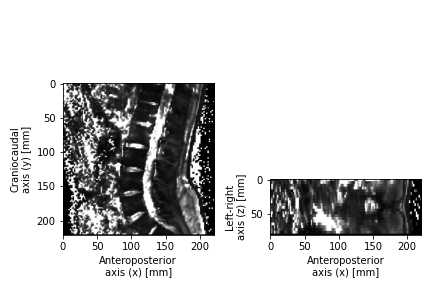
\includegraphics[width=.95\textwidth]{automated_graphs/OSF_02.png}
    \caption{MyoSegmenTUM dataset scan \textit{02}. 
    The volumes are cropped in the left-right direction. 
    \label{fig:OSF_02}}
\end{SCfigure}

\textbf{Remark:} For three volumes (nr 33, 53 and 54) for which the dimension of the image volume and the label mask do not correspond. 
It is not clear how these masks should be used. 
These volumes were discarded, bringing the final number of volumes used from the MyoSegmenTUM dataset to 51.
\subsection{UWSpine dataset}
 
This dataset is made available by the Department of Radiology of the University of Washington\footnote{Creative Commons Attribution-NonCommercial-NoDerivatives 4.0 International License, dataset available at \url{
      https://biomedia.doc.ic.ac.uk/data/spine/  
    }}.
It has been constructed by dr. Glocker and team \cite{Glocker2012,Glocker2013} (Microsoft research) in 2012.
For each scan, manual annotations of vertebrae centroids are provided.
This dataset contains 242 \acrshort{ct} scans of 150 different patients.
This dataset does not contain full mask labels, only centroid point annotations.
To investigate the relative performance of a weakly supervised model compared to the performance of a fully supervised model, both will be trained on the same dataset\footnote{The modelling concept is further discussed in chapter \ref{sec:model_concept}.}.
Furthermore, the evaluation of the models is based on the full annotations.
Thus, the UWSpine dataset will not be used for model training.
It will only be used for visual evaluation of the model on a completely new dataset\footnote{The UWSpine dataset is \textit{completely} new in the sense that no samples from this dataset (this \textit{population}, so to speak) are present in the train or validation set.
For the \textit{normal} test set, other samples from the same datasets where present in the train and validation sets.}.


\subsubsection{Original Objective of the Dataset}

In \cite{Glocker2012,Glocker2013} the development of a model based on regression forests and a \acrfull{hmm} for vertebra localisation without needing strong assumptions on what part of the spine is visible.

\subsubsection{Patient statistics}


Figure \ref{fig:UW_ageboxplot} illustrated that the patients in the \textit{UWSpine} dataset are relatively varied in age.
Of most patients in the dataset, multiple scan images are available.
The highest number of scans taken from a single patient is 5.

\subsubsection{Technical information}

Only point annotations are available for the \textit{UWSpine} dataset. 
This means this dataset can only be used for weakly supervised model training.

The scans in the \textit{UWSpine} dataset are strongly cropped around the spine, both in the left-right direction and the anteroposterior direction.

\begin{SCfigure}[][htb]
    \centering
    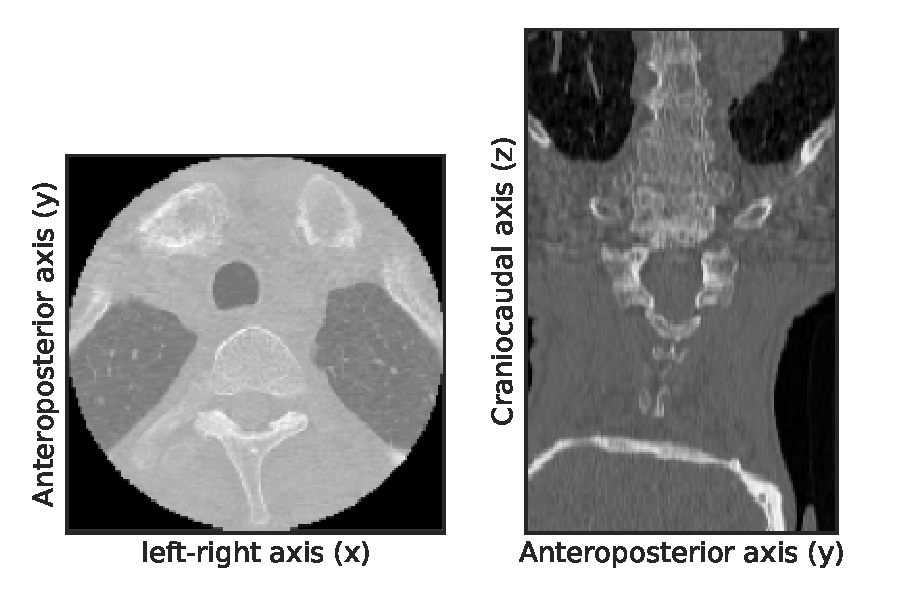
\includegraphics[width=.95\textwidth]{automated_graphs/UW_4564688.pdf}
    \caption{University of Washington dataset, scan \textit{4564688}. \label{fig:UW_4564688}}
\end{SCfigure}

\marginpar{
        % This file was created by tikzplotlib v0.9.8.
\begin{tikzpicture}

\definecolor{color0}{rgb}{0.917647058823529,0.917647058823529,0.949019607843137}
\definecolor{color1}{rgb}{0.298039215686275,0.447058823529412,0.690196078431373}
\definecolor{color2}{rgb}{0.768627450980392,0.305882352941176,0.32156862745098}

\begin{axis}[
axis background/.style={fill=color0},
axis line style={white},
tick align=outside,
tick pos=left,
x grid style={white},
xlabel={Gender},
xmajorgrids,
xmin=0.5, xmax=2.5,
xtick style={color=white!15!black},
xtick={1,2},
xticklabels={Female (54 patients),Male (71 patients)},
y grid style={white},
ylabel={Patient age (y)},
ymajorgrids,
ymin=11.05, ymax=97.95,
ytick style={color=white!15!black}
]
\addplot [color1, opacity=1]
table {%
0.925 42.75
1.075 42.75
1.075 64.75
0.925 64.75
0.925 42.75
};
\addplot [color1, opacity=1]
table {%
1 42.75
1 15
};
\addplot [color1, opacity=1]
table {%
1 64.75
1 94
};
\addplot [black, opacity=1]
table {%
0.9625 15
1.0375 15
};
\addplot [black, opacity=1]
table {%
0.9625 94
1.0375 94
};
\addplot [color1, opacity=1]
table {%
1.925 41.5
2.075 41.5
2.075 65.5
1.925 65.5
1.925 41.5
};
\addplot [color1, opacity=1]
table {%
2 41.5
2 15
};
\addplot [color1, opacity=1]
table {%
2 65.5
2 90
};
\addplot [black, opacity=1]
table {%
1.9625 15
2.0375 15
};
\addplot [black, opacity=1]
table {%
1.9625 90
2.0375 90
};
\addplot [color2, opacity=1]
table {%
0.925 54
1.075 54
};
\addplot [color2, opacity=1]
table {%
1.925 54
2.075 54
};
\end{axis}

\draw ({$(current bounding box.south west)!0.5!(current bounding box.south east)$}|-{$(current bounding box.south west)!0.98!(current bounding box.north west)$}) node[
  scale=0.6,
  anchor=north,
  text=white!15!black,
  rotate=0.0,
  align=center
]{OSF dataset
age distribution};
\end{tikzpicture}

        \captionof{figure}{Distribution of patient age in the dataset from Washington University.}
        \label{fig:UW_ageboxplot}
    }

% Data preparation part
\chapter{Data preprocessing}

The available data volumes have to be preprocessed before being used in the neural network classifier.
The preprocessing steps consist of resampling, slicing, contrast enhancement and cropping.  

There is not one obvious way to combine the different datasets and available labels in one project.
The chosen approach in this work is discussed below.
First, the conversion of the full class labels to point labels is discussed. 
Secondly, the split of the datafiles in a train set, a validation set and a test set is discussed.

\section{Image preprocessing}

A (medical) image\footnote{In this work, I use \textit{image} to refer both to 2-dimensional and 3-dimensional images.} consists of a combination of data - the pixel
\footnote{A \textit{pixel} (picture-element) is the smallest component of a digital bitmap image. 
It is defined by a position vector and carries $c$ values. Where $c$ is the number of channels of the image. 
Sometimes, a pixel of a 3-dimensional digital image is called a \textit{voxel} (volume element).} 
values - and metadata.

For a medical image, there are two types of metadata:
\begin{description}
    \item [Describing the patient \& medical data:] patient identification, pathologies, date of scan, date of birth, gender, weight, height,\dots
    \item [Technical meta-data:] The size (number of pixels per dimension), pixel spacing (distance between pixels along a dimension), orientation vector, image modality \& other information regarding the image acquisition.
\end{description}

For a discussion of the data used in this work, chapter \ref{sec:datasets} can be consulted. 

\subsection{Resampling and slicing\label{sec:resampling}}

In figure \ref{fig:AllDataset_dims}, the differences regarding the dimension and resolution for the different volumes in the combined dataset are illustrated. 
It is necessary to uniformize the data input to the network. 
This requires uniformization of the image spacing vector in all directions\footnote{A typical \acrshort{cnn} is not scale-invariant.}. 
I chose to resample on a $1mm\times 1mm \times 1mm$ isotropic grid. 
If necessary, images are rotated to uniformize the orientation vectors. 
Every image is now a 3-dimensional array\footnote{Both \acrshort{ct} and \acrshort{mri} images have only one channel.} with the same sequence of dimensions and the same spacing along these dimensions.
The chosen uniform dimension sequence is:
\begin{enumerate} 
    \item Craniocaudal axis; perpendicular to the transverse plane.
    \item Anteroposterior axis; perpendicular to the coronal (frontal) plane.
    \item Left-right axis; perpendicular to the sagittal plane.
\end{enumerate}
The inputs for the 2D models are obtained by \textit{slicing} the volume along with one of the dimensions.
This means that from each scan volume, three different sets of two-dimensional slices can be generated, depending on the slicing axis\footnote{The slicing axis is the axis perpendicular to which ones slices the volume}.

When resampling the image itself, linear interpolation is used. 
To resample the classification masks on a new grid, the \textit{nearest neighbour} method is used\footnote{
    SimpleITK \cite{sitk} provides useful tools to perform these operations.
    } 
since factorial data must not be interpolated. 

\subsection{Contrast enhancement}
To two-dimensional images obtained from slicing, the volumes are preprocessed with the \acrfull{clahe} algorithm. 
The difference with ordinary histogram equalization is that the \acrshort{clahe} method calculates different histograms for different sections of the image.
This technique allows improving the local contrast in each region of an image.
When an image contains regions that are significantly lighter or darker than the rest of the image (as is the case for both \acrshort{ct} and \acrshort{mri} images), the AHE methods perform better than histogram equalization based on the complete image.

\begin{SCfigure}[][htb]
    \centering
    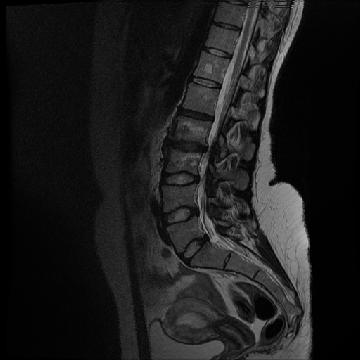
\includegraphics[width=.32\textwidth]{images/orig_usieg8_s22.jpg}
    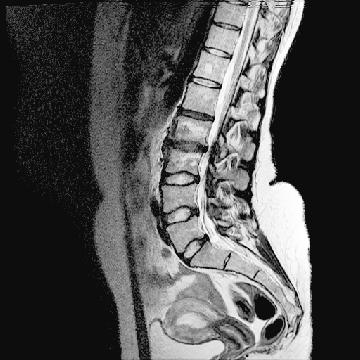
\includegraphics[width=.32\textwidth]{images/hist_usieg8_s22.jpg}
    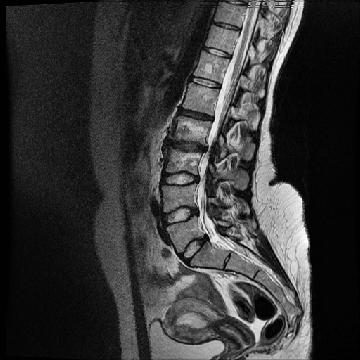
\includegraphics[width=.32\textwidth]{images/clahe_usieg8_s22.jpg}
    \caption{Image: 22$^{th}$ sagittal slice of the 8$^{th}$ image of the USiegen dataset. 
    From left to right, the original image, the image after ordinary histrogram contrast enhancement and the result after \acrshort{clahe}.
    The images show that \acrshort{clahe} avoids increasing the noise in the larger dark areas while resulting in a more balanced image than the ordinary histogram method.
    }
\end{SCfigure}

\acrfull{clahe} is an improvement on adaptive histogram equalization.
Limiting the contrast amplification avoids that noise is amplified in (near) constant regions of the image.
The parameters of this operation were adjusted manually.
Based on trial and error iterations, where the quality of the contrast improvement was estimated with the human eye based on visualizations from all datasets,
the following parameters were chosen:
\begin{description}
    \item[Number of grey bins:] 256 (maximum possible when working with 8-bit encoded images).
    \item[Kernel size:] 50. This parameter defines the extent of the \textit{local} region used by the algorithm.
    \item[clip limit:] $9.10^{-3}$. This parameter suppresses noise in the darkest regions (which contain the least information).
\end{description}

\newpage
\section{Train, validation and test split considerations\label{sec:trainValTestSplit}}

To allow evaluation of the models produced, a test set is split from the development set.
The objective is to evaluate how well a model generalizes to new data\footnote{
    New data is to be interpreted here as a new sample from \textit{the same population} as the development sample.
    Unfortunately, I cannot claim that the different datasets I collected indeed form a perfect representation of the population of medical images of the lumbar spine.}. 
To provide an honest estimate of the out-of-sample performance, the test dataset should represent the investigated population and (hidden) correlations with elements of the development sample should be avoided.

This is done\footnote{
    To accomplish this, I used the function \texttt{GroupedStratifiedSplit} at \url{https://github.com/scikit-learn/scikit-learn/pull/18649/}. 
    This class is not yet part of the official \texttt{sci-kit learn} library release (at the time of writing) but functions well for this application.} taking into account the following:
\begin{description}
    \item[Stratified data:] The combination of data from different sources is stratified. Every source is considered a subpopulation. The data split is made such that the proportion of scans originating from each data source in every split is proportional to their occurrence in the total population.
    \item[Grouped data:] The scans of the same patient can be assumed to be correlated to each other. These scans should not be spread over different splits. The data is split at patient level.
\end{description}

For each datasource, the intended split is $\frac{4}{6}$ for train set, $\frac{1}{6}$ for cross validation set and $\frac{1}{6}$ for test set.
This distribution is not perfect but acceptable, as is indicated by the values in table \ref{tab:summary_split}.

\begin{SCtable}[\sidecaptionrelwidth][h]
 
    \begin{tabular}{lrrr}
\toprule
split &  test &  train &  xval \\
source       &       &        &       \\
\midrule
MyoSegmenTUM &     9 &     33 &     9 \\
PLoS         &     4 &     14 &     4 \\
USiegen      &     2 &     14 &     1 \\
xVertSeg     &     2 &     10 &     3 \\
\bottomrule
\end{tabular}

    \caption{Number of volumes by datasource and by split.\label{tab:summary_split}}
  
  \end{SCtable}

  \begin{SCtable}[\sidecaptionrelwidth][h]
 
    \begin{tabular}{ll|lll|l}
    \toprule
    split        &            & test & train & xval & total \\
    source       & dimension  &      &       &      &       \\ \midrule
    MyoSegmenTUM & Transverse & 1989 & 7293  & 1989 & 11271 \\
                 & Frontal    & 1989 & 7293  & 1989 & 11271 \\
                 & Sagittal   & 720  & 2650  & 725  & 4095  \\
    PLoS         & Transverse & 1528 & 5348  & 1528 & 8404  \\
    USiegen      & Transverse & 733  & 5063  & 501  & 6297  \\
                 & Frontal    & 681  & 4276  & 1080 & 6037  \\
                 & Sagittal   & 145  & 1089  & 180  & 1414  \\
    xVertSeg     & Transverse & 759  & 2652  & 785  & 4196  \\
                 & Frontal    & 812  & 4163  & 1290 & 6265  \\
                 & Sagittal   & 812  & 4163  & 1290 & 6265  \\ \midrule
    total        & Transvers  & 5009 & 20356 & 4803 & 30168 \\
                 & Frontal    & 3482 & 15732 & 4359 & 23573 \\
                 & Sagittal   & 1677 & 7902  & 2195 & 11774 \\ \bottomrule
    \end{tabular}
    \caption{Number of slices by datasource and by split.\label{tab:summary_split_slices}}
  
  \end{SCtable}

The result of this operation is detailed in appendix \ref{sec:appendix_split} on page \pageref{sec:appendix_split}.

\section{Cropping\label{sec:cropping}}
The networks used require input images of size $352 p \times 352 p$, corresponding to $352 mm \times 352 mm$.
The image slices have different dimensions.
The incoming images are cropped or padded, depending on whether the image dimension is smaller or larger than the crop window.


When the image is cropped, one of 5 crops is selected, see figure \ref{fig:crop}:
\begin{description}
    \item[crop 0:] Crop from the top left corner of the image.
    \item[crop 1:] Crop from the top right corner of the image.
    \item[crop 2:] Crop from the bottom left corner of the image.
    \item[crop 3:] Crop from the bottom right corner of the image.
    \item[crop 4:] Center crop of the image.  
\end{description}

Not all slices are sufficiently large to produce 5 different crops. This is illustrated in figure \ref{fig:smallcrop}. In this case, one of the slice dimensions must be padded (symmetrically) to obtain an image of the desired dimensions.

When a slice is fetched from the train set, a random crop is selected from these 5.
This adds an extra level of variance to the training data. This avoids, for example, that the network learns that the spine is always at the same location in the images.

For the slices sourced from the cross-validation and train set, however, reproducibility is essential.
For each slice, the crop number is fixed.
This way, the cross-validation metric, evaluated to avoid overfitting is always calculated on the same images.

When reconstructing the volumes, in the second step of the model concept (see chapter \ref{sec:model_concept}), 
all different crops are evaluated in the model, and the responses for these crops are joined by averaging the model responses in the overlap regions.

\begin{SCfigure}[][htb]
    \centering
    \begin{minipage}{.99\textwidth}
        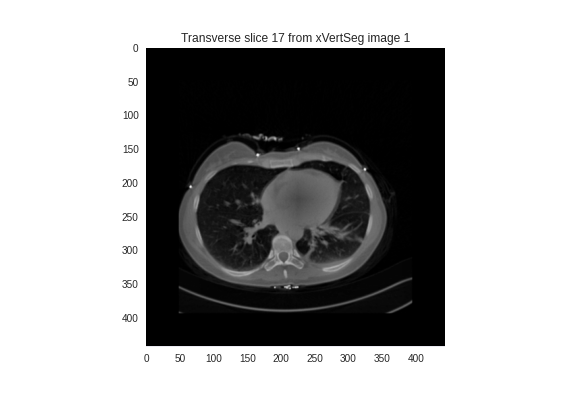
\includegraphics[width=.99\textwidth]{images/slice017.png}
    \end{minipage} 
    \begin{minipage}{0.99\textwidth}
        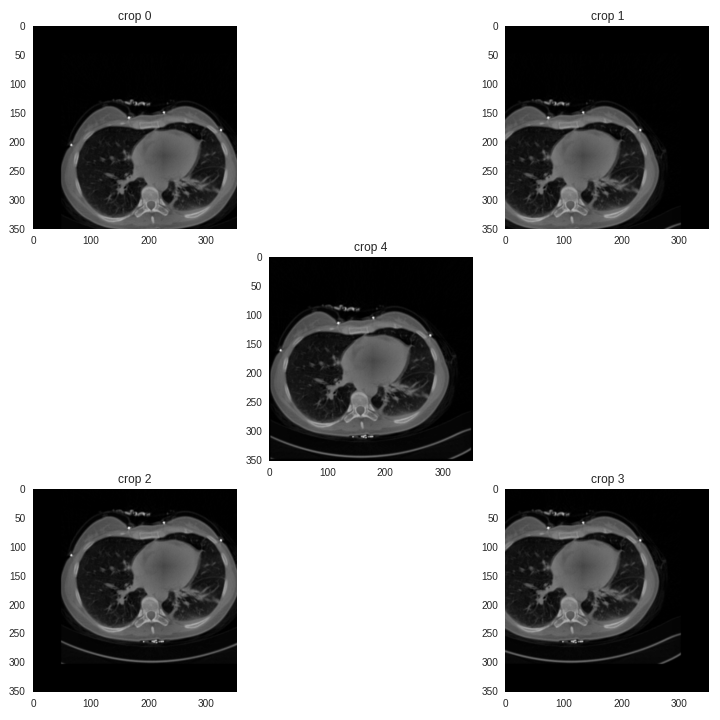
\includegraphics[width=.99\textwidth]{images/cropping_slice017.png}
    \end{minipage}
    \caption{
        Illustration of image cropping where the image is larger than the crop window dimensions. The original size of the image is $443 \times 443$, and the crop window used has dimensions $352 \times 352$.
        Crop 0 to 4 are 5 different images but have a considerable overlap. \label{fig:crop}
        }
    
\end{SCfigure}

\begin{SCfigure}[][htb]
    \centering
    \begin{minipage}{.99\textwidth}
        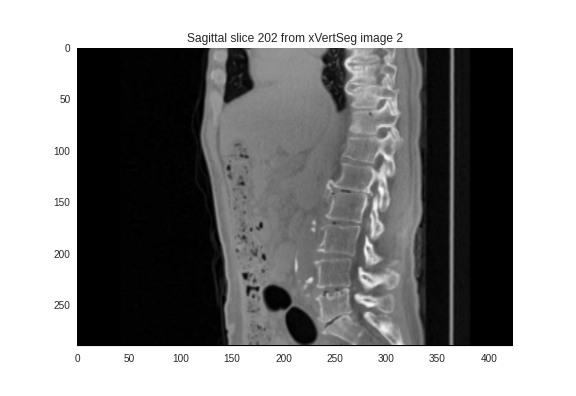
\includegraphics[width=.99\textwidth]{images/slice202.png}
    \end{minipage} 
    \begin{minipage}{0.99\textwidth}
        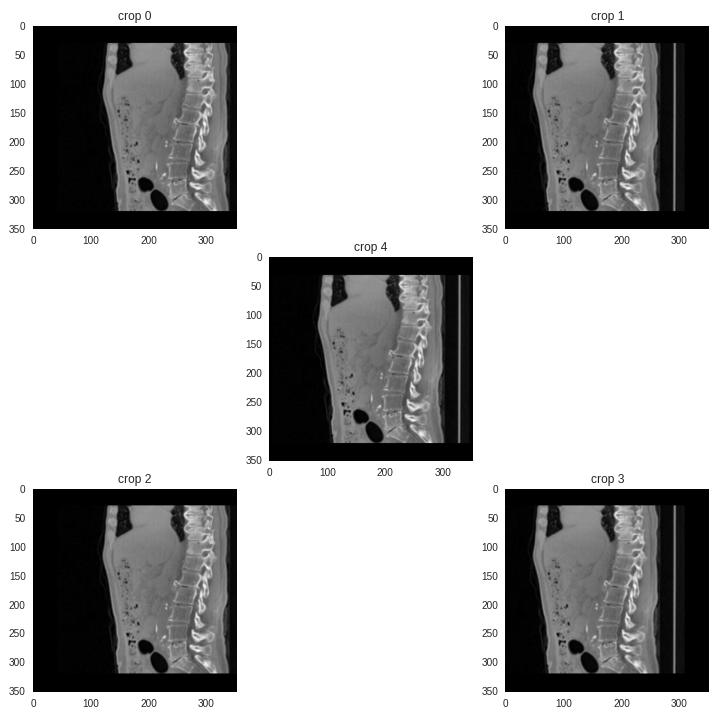
\includegraphics[width=.99\textwidth]{images/cropping_slice202.png}
    \end{minipage}
    \caption{
        Illustration of image cropping where the image is larger than the crop window dimensions.
        The original size of the image is $291 \times 424$, and the crop window used has dimensions $352 \times 352$.
        Crop 0 to 4 are not all different images. Since the image height is lower than the crop window height, this dimension is padded, not cropped.
        This results in crop 0 being equal to crop 2 and crop 1 being equal to crop 3. \label{fig:smallcrop}
        }
    
\end{SCfigure}